% Options for packages loaded elsewhere
\PassOptionsToPackage{unicode}{hyperref}
\PassOptionsToPackage{hyphens}{url}
\documentclass[
  ignorenonframetext,
]{beamer}
\newif\ifbibliography
\usepackage{pgfpages}
\setbeamertemplate{caption}[numbered]
\setbeamertemplate{caption label separator}{: }
\setbeamercolor{caption name}{fg=normal text.fg}
\beamertemplatenavigationsymbolsempty
% remove section numbering
\setbeamertemplate{part page}{
  \centering
  \begin{beamercolorbox}[sep=16pt,center]{part title}
    \usebeamerfont{part title}\insertpart\par
  \end{beamercolorbox}
}
\setbeamertemplate{section page}{
  \centering
  \begin{beamercolorbox}[sep=12pt,center]{section title}
    \usebeamerfont{section title}\insertsection\par
  \end{beamercolorbox}
}
\setbeamertemplate{subsection page}{
  \centering
  \begin{beamercolorbox}[sep=8pt,center]{subsection title}
    \usebeamerfont{subsection title}\insertsubsection\par
  \end{beamercolorbox}
}
% Prevent slide breaks in the middle of a paragraph
\widowpenalties 1 10000
\raggedbottom
\AtBeginPart{
  \frame{\partpage}
}
\AtBeginSection{
  \ifbibliography
  \else
    \frame{\sectionpage}
  \fi
}
\AtBeginSubsection{
  \frame{\subsectionpage}
}
\usepackage{iftex}
\ifPDFTeX
  \usepackage[T1]{fontenc}
  \usepackage[utf8]{inputenc}
  \usepackage{textcomp} % provide euro and other symbols
\else % if luatex or xetex
  \usepackage{unicode-math} % this also loads fontspec
  \defaultfontfeatures{Scale=MatchLowercase}
  \defaultfontfeatures[\rmfamily]{Ligatures=TeX,Scale=1}
\fi
\usepackage{lmodern}
\usetheme[]{Montpellier}
\ifPDFTeX\else
  % xetex/luatex font selection
\fi
% Use upquote if available, for straight quotes in verbatim environments
\IfFileExists{upquote.sty}{\usepackage{upquote}}{}
\IfFileExists{microtype.sty}{% use microtype if available
  \usepackage[]{microtype}
  \UseMicrotypeSet[protrusion]{basicmath} % disable protrusion for tt fonts
}{}
\makeatletter
\@ifundefined{KOMAClassName}{% if non-KOMA class
  \IfFileExists{parskip.sty}{%
    \usepackage{parskip}
  }{% else
    \setlength{\parindent}{0pt}
    \setlength{\parskip}{6pt plus 2pt minus 1pt}}
}{% if KOMA class
  \KOMAoptions{parskip=half}}
\makeatother
\usepackage{color}
\usepackage{fancyvrb}
\newcommand{\VerbBar}{|}
\newcommand{\VERB}{\Verb[commandchars=\\\{\}]}
\DefineVerbatimEnvironment{Highlighting}{Verbatim}{commandchars=\\\{\}}
% Add ',fontsize=\small' for more characters per line
\usepackage{framed}
\definecolor{shadecolor}{RGB}{248,248,248}
\newenvironment{Shaded}{\begin{snugshade}}{\end{snugshade}}
\newcommand{\AlertTok}[1]{\textcolor[rgb]{0.94,0.16,0.16}{#1}}
\newcommand{\AnnotationTok}[1]{\textcolor[rgb]{0.56,0.35,0.01}{\textbf{\textit{#1}}}}
\newcommand{\AttributeTok}[1]{\textcolor[rgb]{0.13,0.29,0.53}{#1}}
\newcommand{\BaseNTok}[1]{\textcolor[rgb]{0.00,0.00,0.81}{#1}}
\newcommand{\BuiltInTok}[1]{#1}
\newcommand{\CharTok}[1]{\textcolor[rgb]{0.31,0.60,0.02}{#1}}
\newcommand{\CommentTok}[1]{\textcolor[rgb]{0.56,0.35,0.01}{\textit{#1}}}
\newcommand{\CommentVarTok}[1]{\textcolor[rgb]{0.56,0.35,0.01}{\textbf{\textit{#1}}}}
\newcommand{\ConstantTok}[1]{\textcolor[rgb]{0.56,0.35,0.01}{#1}}
\newcommand{\ControlFlowTok}[1]{\textcolor[rgb]{0.13,0.29,0.53}{\textbf{#1}}}
\newcommand{\DataTypeTok}[1]{\textcolor[rgb]{0.13,0.29,0.53}{#1}}
\newcommand{\DecValTok}[1]{\textcolor[rgb]{0.00,0.00,0.81}{#1}}
\newcommand{\DocumentationTok}[1]{\textcolor[rgb]{0.56,0.35,0.01}{\textbf{\textit{#1}}}}
\newcommand{\ErrorTok}[1]{\textcolor[rgb]{0.64,0.00,0.00}{\textbf{#1}}}
\newcommand{\ExtensionTok}[1]{#1}
\newcommand{\FloatTok}[1]{\textcolor[rgb]{0.00,0.00,0.81}{#1}}
\newcommand{\FunctionTok}[1]{\textcolor[rgb]{0.13,0.29,0.53}{\textbf{#1}}}
\newcommand{\ImportTok}[1]{#1}
\newcommand{\InformationTok}[1]{\textcolor[rgb]{0.56,0.35,0.01}{\textbf{\textit{#1}}}}
\newcommand{\KeywordTok}[1]{\textcolor[rgb]{0.13,0.29,0.53}{\textbf{#1}}}
\newcommand{\NormalTok}[1]{#1}
\newcommand{\OperatorTok}[1]{\textcolor[rgb]{0.81,0.36,0.00}{\textbf{#1}}}
\newcommand{\OtherTok}[1]{\textcolor[rgb]{0.56,0.35,0.01}{#1}}
\newcommand{\PreprocessorTok}[1]{\textcolor[rgb]{0.56,0.35,0.01}{\textit{#1}}}
\newcommand{\RegionMarkerTok}[1]{#1}
\newcommand{\SpecialCharTok}[1]{\textcolor[rgb]{0.81,0.36,0.00}{\textbf{#1}}}
\newcommand{\SpecialStringTok}[1]{\textcolor[rgb]{0.31,0.60,0.02}{#1}}
\newcommand{\StringTok}[1]{\textcolor[rgb]{0.31,0.60,0.02}{#1}}
\newcommand{\VariableTok}[1]{\textcolor[rgb]{0.00,0.00,0.00}{#1}}
\newcommand{\VerbatimStringTok}[1]{\textcolor[rgb]{0.31,0.60,0.02}{#1}}
\newcommand{\WarningTok}[1]{\textcolor[rgb]{0.56,0.35,0.01}{\textbf{\textit{#1}}}}
\setlength{\emergencystretch}{3em} % prevent overfull lines
\providecommand{\tightlist}{%
  \setlength{\itemsep}{0pt}\setlength{\parskip}{0pt}}
%\documentclass[unicode,10pt]{beamer}% 'unicode'が必要
\usepackage{luatexja}% 日本語を使う場合は必須
%\usepackage[japanese]{babel}	
%\usefonttheme[onlymath]{serif}
%\usepackage[T1]{fontenc} %これを使うと、ギリシャ文字が出ない
%\usepackage{textcomp}
%\usepackage[scale=1.0]{tgheros} % Sans serif font
%\usepackage[scaled]{beramono} % Monospace font
%\usepackage{luatexja-otf}
%\renewcommand{\kanjifamilydefault}{\gtdefault}
%\usepackage[haranoaji]{luatexja-preset}

% スライド番号の表示 %%%%%%%%%%%%%%%%%%%
\makeatletter
\setbeamertemplate{footline}{%
  \leavevmode%
  \hbox{%
  \begin{beamercolorbox}[wd=.5\paperwidth,ht=2.25ex,dp=1ex,right]{date in head/foot}%
    \insertframenumber{} \hspace*{2ex} % new version without total frames
  \end{beamercolorbox}}%
  \vskip0pt%
}
\makeatother
% スライド番号の表示 %%%%%%%%%%%%%%%%%%%
\usepackage{bookmark}
\IfFileExists{xurl.sty}{\usepackage{xurl}}{} % add URL line breaks if available
\urlstyle{same}
\hypersetup{
  hidelinks,
  pdfcreator={LaTeX via pandoc}}

\title{第5章: 説明（観察データによる因果効果の推定）}
\subtitle{Elena Llaudet \& Kosuke Imai.\\
Data Analysis for Social Science: A Friendly and Practical
Introduction.}
\author{}
\date{\vspace{-2.5em}2026-03-09}

\begin{document}
\frame{\titlepage}

\section{5.1
観察研究と共変量}\label{ux89b3ux5bdfux7814ux7a76ux3068ux5171ux5909ux91cf}

\begin{frame}{観察研究 (Observational Studies)}
\phantomsection\label{ux89b3ux5bdfux7814ux7a76-observational-studies}
\begin{itemize}
\tightlist
\item
  研究者が処置を無作為に割り当て\textbf{ない}研究。
\item
  \textbf{メリット}: 倫理的・物理的な理由で実験できない現象も分析可能。
\item
  \textbf{デメリット}: \textbf{共変量} (Confounders)
  によるバイアスが発生しやすい。
\end{itemize}
\end{frame}

\begin{frame}{共変量 (Confounders)}
\phantomsection\label{ux5171ux5909ux91cf-confounders}
\begin{itemize}
\tightlist
\item
  処置 (\(X\)) と結果 (\(Y\)) の両方に影響を与える変数。
\item
  これにより、処置群と統制群が「平均的に同一」ではなくなり、単純な平均の差では因果効果を測定できなくなる。
\end{itemize}
\end{frame}

\section{5.2 重回帰分析 (Multiple
Regression)}\label{ux91cdux56deux5e30ux5206ux6790-multiple-regression}

\begin{frame}{なぜ重回帰か？}
\phantomsection\label{ux306aux305cux91cdux56deux5e30ux304b}
\begin{itemize}
\tightlist
\item
  単純な回帰 (\(\hat{Y} = \hat{\alpha} + \hat{\beta} X\))
  では、他の要因を考慮できない。
\item
  \textbf{重回帰}では、複数の独立変数を同時にモデルに含めることができる。
\item
  数式:
  \(\hat{Y} = \hat{\alpha} + \hat{\beta}_1 X_1 + \hat{\beta}_2 X_2 + \dots\)
\item
  これにより、「\(X_2\)
  などの\textbf{他の要因を一定に保ったまま}、\(X_1\) が \(Y\)
  に与える影響」を推定できる。
\end{itemize}
\end{frame}

\section{5.3
データの読み込みと準備}\label{ux30c7ux30fcux30bfux306eux8aadux307fux8fbcux307fux3068ux6e96ux5099}

\begin{frame}[fragile]{ウクライナの選挙データ}
\phantomsection\label{ux30a6ux30afux30e9ux30a4ux30caux306eux9078ux6319ux30c7ux30fcux30bf}
\begin{itemize}
\tightlist
\item
  2014年ウクライナ議会選挙のデータ。
\item
  \textbf{関心}:
  ロシアのテレビ放送を視聴できることが、親ロシア派への投票に与える影響。
\end{itemize}

\begin{Shaded}
\begin{Highlighting}[]
\CommentTok{\# データの読み込み}
\NormalTok{precincts }\OtherTok{\textless{}{-}} \FunctionTok{read.csv}\NormalTok{(}\StringTok{"UA\_precincts.csv"}\NormalTok{)}
\CommentTok{\# 最初の数行を表示}
\FunctionTok{head}\NormalTok{(precincts)}
\end{Highlighting}
\end{Shaded}

\begin{verbatim}
##   russian_tv pro_russian prior_pro_russian within_25km
## 1          0   2.7210884          25.14286           1
## 2          0   0.8928571          35.34483           0
## 3          1   1.6949153          20.53232           1
## 4          0  72.2689076          84.47761           1
## 5          0   1.2820513          28.99408           0
## 6          1   1.4285714          45.58824           0
\end{verbatim}
\end{frame}

\section{5.4 共変量の制御}\label{ux5171ux5909ux91cfux306eux5236ux5fa1}

\begin{frame}[fragile]{ロシア放送の影響}
\phantomsection\label{ux30edux30b7ux30a2ux653eux9001ux306eux5f71ux97ff}
\begin{itemize}
\tightlist
\item
  単純に比較すると、ロシア放送を受信できる地域は、もともと親ロシア的な傾向が強い可能性がある（交絡）。
\item
  そこで、\textbf{過去の投票率} (\texttt{prior\_pro\_russian})
  を制御変数として追加する。
\end{itemize}
\end{frame}

\begin{frame}[fragile]{ロシア放送の影響: Rコード}
\phantomsection\label{ux30edux30b7ux30a2ux653eux9001ux306eux5f71ux97ff-rux30b3ux30fcux30c9}
\footnotesize

\begin{Shaded}
\begin{Highlighting}[]
\CommentTok{\# 重回帰モデルの推定}
\NormalTok{model\_mult }\OtherTok{\textless{}{-}} \FunctionTok{lm}\NormalTok{(pro\_russian }\SpecialCharTok{\textasciitilde{}}\NormalTok{ russian\_tv }\SpecialCharTok{+}\NormalTok{ prior\_pro\_russian, }
                 \AttributeTok{data =}\NormalTok{ precincts)}
\CommentTok{\# 結果の表示}
\FunctionTok{summary}\NormalTok{(model\_mult)}
\end{Highlighting}
\end{Shaded}

\begin{verbatim}
## 
## Call:
## lm(formula = pro_russian ~ russian_tv + prior_pro_russian, data = precincts)
## 
## Residuals:
##     Min      1Q  Median      3Q     Max 
## -38.776  -7.569   0.154   7.346  26.007 
## 
## Coefficients:
##                     Estimate Std. Error t value Pr(>|t|)    
## (Intercept)       -13.795374   0.525786  -26.24   <2e-16 ***
## russian_tv          5.004216   0.484348   10.33   <2e-16 ***
## prior_pro_russian   0.767525   0.009919   77.38   <2e-16 ***
## ---
## Signif. codes:  0 '***' 0.001 '**' 0.01 '*' 0.05 '.' 0.1 ' ' 1
## 
## Residual standard error: 11.01 on 3586 degrees of freedom
## Multiple R-squared:  0.6651, Adjusted R-squared:  0.6649 
## F-statistic:  3561 on 2 and 3586 DF,  p-value: < 2.2e-16
\end{verbatim}

\normalsize
\end{frame}

\begin{frame}[fragile]{推定値の解釈}
\phantomsection\label{ux63a8ux5b9aux5024ux306eux89e3ux91c8}
\begin{itemize}
\tightlist
\item
  \texttt{russian\_tv} の係数:
  過去の投票率を一定に保ったとき、ロシア放送が受信可能であることで、今回の親ロシア派の得票率が平均で何\%変化したか。
\end{itemize}
\end{frame}

\section{5.5
回帰モデルの比較}\label{ux56deux5e30ux30e2ux30c7ux30ebux306eux6bd4ux8f03}

\begin{frame}[fragile]{モデル間の比較}
\phantomsection\label{ux30e2ux30c7ux30ebux9593ux306eux6bd4ux8f03}
\begin{itemize}
\tightlist
\item
  制御変数を入れる前と後で係数がどう変わるかを確認する。
\end{itemize}

\footnotesize

\begin{Shaded}
\begin{Highlighting}[]
\CommentTok{\# 単純回帰}
\NormalTok{model\_sim }\OtherTok{\textless{}{-}} \FunctionTok{lm}\NormalTok{(pro\_russian }\SpecialCharTok{\textasciitilde{}}\NormalTok{ russian\_tv, }\AttributeTok{data =}\NormalTok{ precincts)}
\FunctionTok{coef}\NormalTok{(model\_sim)[}\StringTok{"russian\_tv"}\NormalTok{]}
\end{Highlighting}
\end{Shaded}

\begin{verbatim}
## russian_tv 
##   15.64044
\end{verbatim}

\begin{Shaded}
\begin{Highlighting}[]
\CommentTok{\# 重回帰（過去の投票率を制御）}
\FunctionTok{coef}\NormalTok{(model\_mult)[}\StringTok{"russian\_tv"}\NormalTok{]}
\end{Highlighting}
\end{Shaded}

\begin{verbatim}
## russian_tv 
##   5.004216
\end{verbatim}

\normalsize
\end{frame}

\section{5.6
散布図と回帰平面（視覚化）}\label{ux6563ux5e03ux56f3ux3068ux56deux5e30ux5e73ux9762ux8996ux899aux5316}

\begin{frame}[fragile]{3次元的な関係の理解}
\phantomsection\label{ux6b21ux5143ux7684ux306aux95a2ux4fc2ux306eux7406ux89e3}
\begin{itemize}
\tightlist
\item
  複数の変数の関係をプロットする。
\end{itemize}

\footnotesize

\begin{Shaded}
\begin{Highlighting}[]
\CommentTok{\# 高度な可視化の代わりに、制御変数ごとの回帰直線を確認（概念図）}
\FunctionTok{plot}\NormalTok{(precincts}\SpecialCharTok{$}\NormalTok{prior\_pro\_russian, precincts}\SpecialCharTok{$}\NormalTok{pro\_russian,}
     \AttributeTok{col =} \FunctionTok{ifelse}\NormalTok{(precincts}\SpecialCharTok{$}\NormalTok{russian\_tv }\SpecialCharTok{==} \DecValTok{1}\NormalTok{, }\StringTok{"red"}\NormalTok{, }\StringTok{"blue"}\NormalTok{),}
     \AttributeTok{xlab =} \StringTok{"Prior Pro{-}Russian Vote"}\NormalTok{, }
     \AttributeTok{ylab =} \StringTok{"Current Pro{-}Russian Vote"}\NormalTok{,}
     \AttributeTok{main =} \StringTok{"Regression with Control Variable"}\NormalTok{)}
\FunctionTok{legend}\NormalTok{(}\StringTok{"topleft"}\NormalTok{, }\AttributeTok{legend =} \FunctionTok{c}\NormalTok{(}\StringTok{"Russian TV"}\NormalTok{, }\StringTok{"No Russian TV"}\NormalTok{), }
       \AttributeTok{col =} \FunctionTok{c}\NormalTok{(}\StringTok{"red"}\NormalTok{, }\StringTok{"blue"}\NormalTok{), }\AttributeTok{pch =} \DecValTok{1}\NormalTok{)}
\end{Highlighting}
\end{Shaded}

\begin{center}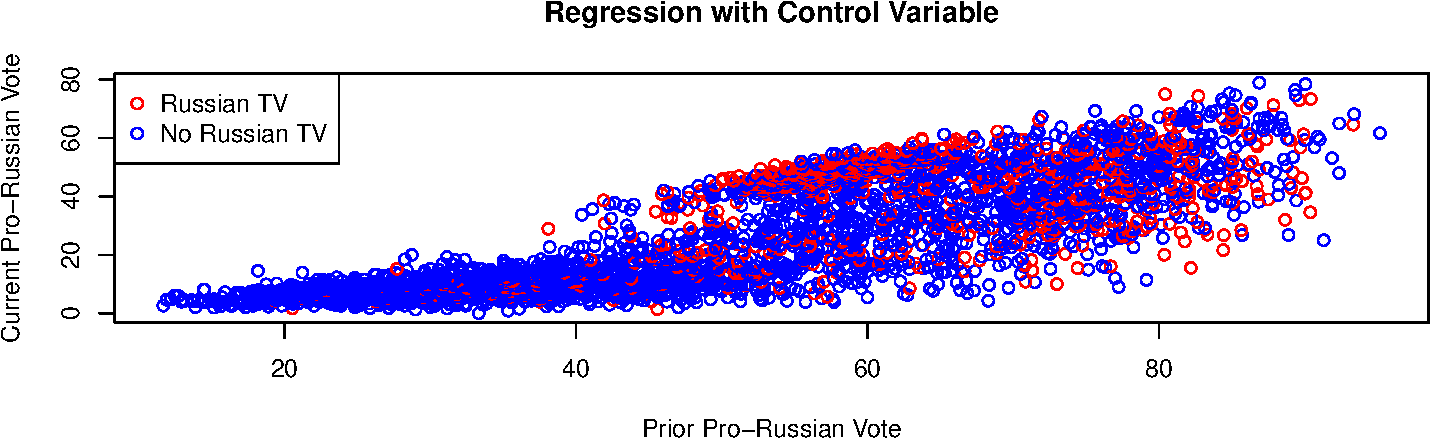
\includegraphics[height=0.3\textheight]{DSS_Ch05_files/figure-beamer/unnamed-chunk-4-1} \end{center}

\normalsize
\end{frame}

\section{5.7 まとめ}\label{ux307eux3068ux3081}

\begin{frame}{第5章のまとめ}
\phantomsection\label{ux7b2c5ux7ae0ux306eux307eux3068ux3081}
\begin{itemize}
\tightlist
\item
  \textbf{観察研究}では、共変量（交絡因子）の存在を常に警戒する必要がある。
\item
  \textbf{重回帰分析}を用いることで、他の要因を「一定に保つ（コントロールする）」ことができる。
\item
  適切な制御変数を含めることで、観察データからも、より信頼性の高い因果効果の推定が可能になる。
\item
  ただし、\textbf{観察されていない共変量}によるバイアスの可能性は常に残る。
\end{itemize}
\end{frame}

\end{document}
